\documentclass[tikz]{standalone}
\usepackage{tikz}
\usetikzlibrary{fit}
\usepackage[dvipsnames]{xcolor}
\usetikzlibrary{positioning, arrows.meta, calc, decorations.pathreplacing}
\definecolor{lightblue}{RGB}{173, 216, 230}
\begin{document}
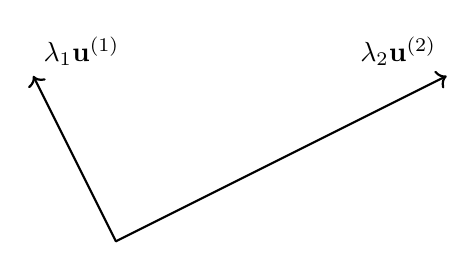
\begin{tikzpicture}[scale=2.1, line cap=round, line join=round]
            % two eigenvectors with different lengths
            \draw[->, thick] (0,0) -- (-0.5,1) node[above right] {$\lambda_{1} {\bf u}^{(1)}$};
            \draw[->, thick] (0,0) -- (2.0,1) node[above left]  {$\lambda_{2} {\bf u}^{(2)}$};
            \end{tikzpicture}
\end{document}
